\subsection{Certified accuracy budgets beyond window resolution}
\label{ssec:certified-accuracy-budget}

Window membership and digit accuracy require different mode budgets.
The preceding finite interlacing yields an exact accuracy threshold
when a terminal analytic root lies strictly above its reference.
Throughout this subsection the source is the \emph{zero-shift} pencil;
the ground correction is treated separately below.

\begin{proposition}[Finite one-sided accuracy threshold]
\label{prop:finite-accuracy-threshold}
Let a common positive analytic source and its prefixes satisfy
Proposition~\ref{prop:prefix-count-interlacing}, with all generalized
squared roots positive. Suppose
$\nu^{(0)}_{k,M}>\gamma_k$. For $k\le N\le M$ and $d>0$, set
$b_{k,d}=\gamma_k(1+10^{-d})$. Then
\[
 0<\frac{\nu^{(0)}_{k,N}-\gamma_k}{\gamma_k}<10^{-d}
 \quad\Longleftrightarrow\quad
 \#\{j:\nu^{(0)}_{j,N}<b_{k,d}\}\ge k.
\]
The accuracy event is monotone in $N$ over this finite family. Its first
occurrence, if any, is certified by counts at two adjacent mode sizes.
\end{proposition}
\begin{proof}
Interlacing gives $\nu^{(0)}_{k,N}\ge\nu^{(0)}_{k,M}>\gamma_k$.
The remaining strict upper inequality is equivalent to the stated
ordinal count, which is monotone in $N$ by the same interlacing.
\end{proof}

The analytic terminal-root certificates establish this positivity
premise for every $k=1,\ldots,1000$ at $(C,M)=(125,2000)$ and
$(250,1500)$. Two exact decimal endpoints guard each reference-based
threshold by $10^{-6}$ times its requested absolute tolerance. The
indexed source inequalities in Section~\ref{ssec:certified-prefix-transfer}
verify that the lower endpoint remains below the threshold and the
upper endpoint above it after analytic source perturbation. Equal
entry indices at the two guards therefore certify the exact integer
minimum. Equality, unresolved arithmetic and a non-reached tolerance
are distinct outcomes; none is rounded into a pass.

\begin{center}
\begin{tabular}{r|rr|rr}
\toprule
 & \multicolumn{2}{c|}{$C=125,\ M=2000$} & \multicolumn{2}{c}{$C=250,\ M=1500$} \\
Depth $d$ & prefix $K$ & minimum $N$ & prefix $K$ & minimum $N$ \\
\midrule
6 & 1000 & 1092 & 1000 & 1220 \\
12 & 1000 & 1103 & 1000 & 1226 \\
25 & 989 & 1239 & 1000 & 1235 \\
50 & 896 & 1212 & 1000 & 1246 \\
100 & 753 & 1201 & 1000 & 1262 \\
250 & 456 & 1323 & 1000 & 1406 \\
500 & 127 & 1179 & 734 & 1500 \\
750 & 0 & -- & 407 & 1500 \\
1000 & 0 & -- & 133 & 1496 \\
\bottomrule
\end{tabular}
\end{center}

Here $K$ is the complete prefix attaining the requested relative
accuracy within the tested family, and $N$ is the smallest common
budget for that prefix. All 18\,000 targets are retained: 12\,495
have certified exact integer minima and 5505 do not reach the tolerance
through their tested maximum. No final target is unresolved. At $C=250$,
13\,371 endpoint attempts require refinement from 3500 to 5000 decimal
working digits; the failed first attempts are retained. These are
evaluation precisions for this certificate, not necessary bit-$P$ limits.

The full unfitted action inversion remains imperfect. At $C=125$,
the 25-digit model misses 14 reachable targets; at 500 digits it
underbudgets 92 of the 127 mutually reachable targets, by as many as
19 modes, and predicts one additional target not reached by $N=2000$.
At $C=250$, the six-digit budget is insufficient at three indices;
at 1000 digits it underbudgets 112 of 133 mutually reachable targets,
by as many as 11 modes. All non-reach outcomes are included in the
comparison. These discrepancies concern the required number of modes,
not the relative error of a displacement predictor.

\begin{figure}[htbp]
\centering
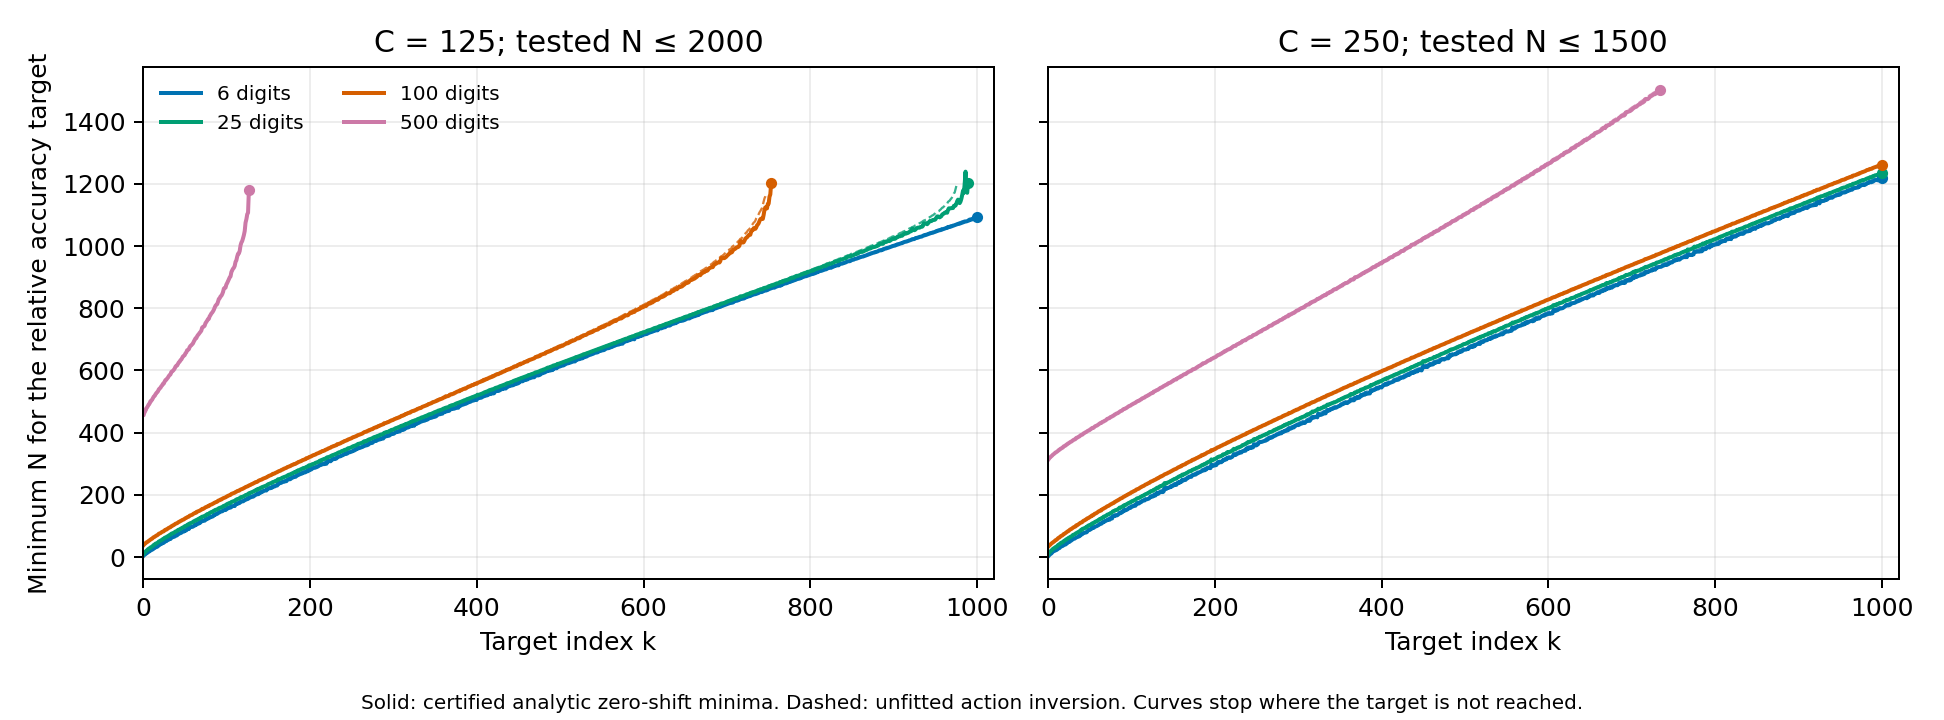
\includegraphics[width=\linewidth]{figures/accuracy_budgets.png}
\caption{Specified-accuracy mode budgets for the finite analytic
zero-shift pencils. The cutoff and requested depth change both the
reachable prefix and its mode requirement. No fixed integer padding
has been fitted.}
\label{fig:accuracy-budgets}
\end{figure}



For a complete prefix through $K$, the required budget is the maximum
of the individual minima through $K$, not automatically the minimum
for index $K$ alone. A target not reached at the tested maximum $M$
fails at all smaller mode sizes in this family. This does not establish
failure for $N>M$ or in the infinite-mode limit. The count benchmark
uses reference ordinates to assess accuracy; it is not itself a
reference-free prediction law.

\paragraph{An unfitted additional-mode term.}
There is a useful local inversion of the previously derived continuum
action. For fixed $C$, $L=\log C$ and $4\pi<x<4\pi C$, put
\[
 u=\frac{\pi\log(x/(4\pi))}{2L},\quad
 N_0=\frac{xL\sin u}{2\pi},\quad b_0=x\cos u,\quad
 K_0=1+\frac{2L}{\pi}\tan u.
\]
Implicit differentiation of the model endpoint equation at $a=x$
gives $a'(N_0)=4x/(b_0K_0)$. The model action consequently obeys
\[
 S(C,N_0+\Delta,x)
 =\frac{16\sqrt2\,x}{3b_0^{3/2}\sqrt{K_0}}\Delta^{3/2}
       +o(\Delta^{3/2}).
\]
Its local inverse at small depth is
\[
 N_{\rm model}(C,x,d)=N_0+
 x^{1/3}\cos u\,K_0^{1/3}
 \left(\frac{3\log10}{16\sqrt2}\right)^{2/3}d^{2/3}
 +o(d^{2/3}).
\]
This coefficient is derived, not fitted. The expansion is nonuniform
as $u\to\pi/2$ and is not presumed accurate even at six digits.
The comparison above inverts the full implicit action, with the degree
floor $N\ge k$; it does not substitute this local expansion. There are
160 numerical model-identity and limiting checks on 20 fixtures,
separate from the analytic CCM count certificates.

If a bound $|D_N-S_N/\log10|\le B$ were established, the actual integer
budget would lie between the model inverse budgets at $d-B$ and $d+B$,
with endpoint and degree conventions retained. Locally,
\[
 \Delta N\simeq\frac{\log10\,\Delta D}{\partial_NS}.
\]
Thus a modest missing amplitude in digit space can produce a substantial
budget error when the action slope is small. Beyond its formal fixed-$C$
cap the model slope is zero while the finite pencil still changes with
$N$. Neither an empirical padding nor a minimum term alone supplies
the missing amplitude and finite-mode tail. The ground correction,
indexed numerical error and limiting identification remain necessary
for the requested $C,N,P,k$ convergence law.
